\section{Introducción}
\subsection{Maple Flow}
Maple Flow es una nueva herramienta de cálculo de Maplesoft. Maple Flow ofrece una interfaz de usuario de forma libre combinada con un motor matemático integral. Utilice Maple Flow para cálculos y documentación de ingeniería, científicos y técnicos.

\newp

Maple Flow te da:

\begin{itemize}
	\item Un lienzo matemático espacialmente consciente que replica la metáfora del diseño de una pizarra física
	
	\item Recálculo automático para garantizar que los resultados estén siempre actualizados
	
	\item Un lenguaje matemático amplio y rico con muchas funciones
	
	\item Tramas visualmente impactantes, completamente programáticas
	
	\item Una región de codificación con acceso completo al lenguaje de programación Maple
	
\end{itemize}

Nota para usuarios que no son de Windows: Las pulsaciones de teclas que se dan en este documento son para Windows. Si está utilizando una plataforma diferente, consulte los métodos abreviados de teclado para su plataforma en Métodos abreviados de teclado (página 34).

\subsection{¿Qué pretende hacer este manual?}
Este manual describe

\begin{itemize}
  \item La interfaz Maple Flow
  
  \item Diferencias con la interfaz de usuario de Maple y el lenguaje de programación que un usuario existente de Maple puede experimentar.

\end{itemize}

Este manual debe leerse al unísono con los tutoriales y ejercicios del producto; estos están disponibles en el enlace Tutorial en la página de inicio de Maple Flow. Si ha cerrado la página de inicio, puede volver a acceder a ella desde el menú Ver:

\begin{itemize}
  \item Seleccione Ver $>$ Inicio Tutorial		
\end{itemize}

\insertimage[]{2022_12_20_3e2ffe6ad124ec91ee5cg-08}{width=10cm}{Descripción general de los tutoriales del producto.}	

Este manual no describe la funcionalidad matemática de Maple Flow en detalle, pero hace referencia a funciones específicas en el contexto de una discusión más amplia. La documentación detallada de la funcionalidad matemática se encuentra en la ayuda en línea de Maple: \href{http://www.maplesoft.com/support/help}{http://www.maplesoft.com/support/help}.

\subsection{¿Cuál es la relación entre Maple y Maple Flow?}
Primero, algunas definiciones:

\begin{itemize}
	\item Maple se refiere al (i) lenguaje de programación Maple y (ii) la interfaz Maple.

	\item Maple Flow se refiere al nuevo producto cuyo manual está leyendo.
\end{itemize}

Maple Flow

\begin{itemize}
  \item Está construido sobre el lenguaje de programación Maple
  
  \item Toma prestados algunos elementos de la interfaz de Maple
\end{itemize}

El "lenguaje" de Maple Flow son los comandos (y su sintaxis), las estructuras de datos y el lenguaje de programación. Estos se basan en el lenguaje de programación Maple; puede utilizar cualquiera de las funciones matemáticas de Maple en sus análisis de Maple Flow.

Maple se instala automáticamente cuando instala Maple Flow.

\subsection{Si eres usuario de Maple}
Si ya usa Maple, apreciará el giro único que ofrece Maple Flow con su modelo de evaluación espacial y las actualizaciones automáticas de cálculo. También obtendrá una ventaja inicial porque estará familiarizado con el lenguaje de programación, las funciones y las características de Maple.

Maple Flow se diferencia de la interfaz y el lenguaje de programación de Maple en varios aspectos. Varias diferencias importantes se enumeran en la Tabla 1.1.

\insertimage[]{2022_12_20_3e2ffe6ad124ec91ee5cg-09}{width=\textwidth}{Tabla 1.1: En qué se diferencia Maple Flow de Maple.}

Las hojas de trabajo de Maple no se pueden cargar en Maple Flow, o viceversa.

\subsection{Sistema de ayuda Maple Flow}
El sistema de ayuda del producto, al que se accede a través del menú Ayuda, proporciona información sobre más de 130 comandos clave. Cada página de ayuda brinda detalles sobre el uso de un comando, incluida la secuencia de llamada, los parámetros, las opciones y los ejemplos.

Buscar: busque un nombre de comando, una palabra clave o una frase.

Examinar: explore la tabla de contenido para ver una lista estructurada de temas de ayuda

Ver página de ayuda como hoja de trabajo: puede abrir cualquier página de ayuda como hoja de trabajo para interactuar con la página y modificar los ejemplos.

\begin{itemize}
  \item Con la página de ayuda mostrada en el panel derecho del sistema de ayuda, desde el menú Ver, seleccione Abrir página como hoja de trabajo. Se abre una nueva ventana de hoja de cálculo. 
  \item Como alternativa, haga clic en Abrir la página actual como hoja de trabajo (ws) en la barra de herramientas del sistema de ayuda.
\end{itemize}

\textbf{Documentación adicional}
Dado que Maple Flow utiliza el lenguaje de programación Maple, tiene la capacidad de utilizar la amplia funcionalidad matemática que forma parte del lenguaje de programación Maple. Al navegar por el sistema de ayuda, algunos hipervínculos lo llevan a documentación detallada adicional para la funcionalidad matemática que reside en el sitio web de Maplesoft, en la ayuda en línea de Maple:

\href{http://www.maplesoft.com/support/help}{http://www.maplesoft.com/support/help}. Tenga en cuenta que estas páginas están formateadas como páginas de Maple, no como páginas de Maple Flow, por lo que los ejemplos se verán un poco diferentes.

\subsection{Interfaz}
Las diferentes partes de la interfaz Maple Flow, como se ve en la Figura 1.2, son:

\begin{itemize}
  \item Canvas - el espacio de trabajo

\item Barra de herramientas principal - Esta barra de herramientas siempre está en la parte superior de la ventana de Maple Flow.

\item Barra de herramientas contextual: esta barra de herramientas, ubicada directamente sobre el lienzo, es relevante para la selección actual.

\item Paletas : en el panel izquierdo, proporcionan una manera fácil de ingresar una expresión matemática, matriz, letra griega o unidades.

\item Panel de contexto: aquí aparecen algunas opciones relevantes para la selección actual, como formato numérico y formato de unidades.

\item Barra de estado — Muestra información del sistema
\end{itemize}
\insertimage[\label{img::1.2}]{ 2022_12_20_3e2ffe6ad124ec91ee5cg-10}{width=17cm}{La interfaz Maple Flow.}

\textbf{Personalizar la interfaz}
Personalice sus preferencias de Maple Flow utilizando el cuadro de diálogo Opciones.

Para abrir el cuadro de diálogo Opciones:

\begin{itemize}
  \item En la barra de herramientas, haga clic en el icono Opciones ( $\boldsymbol{*})$. Hay dos pestañas. En la pestaña Mostrar, puede especificar el número predeterminado de lugares decimales para usar al redondear los resultados. Para obtener más información, consulte Formato numérico (página 10).
\end{itemize}

En la pestaña Interfaz, puede especificar lo siguiente:

\begin{itemize}
  \item Abrir hojas de trabajo en una nueva pestaña o nueva ventana.

\item Abrir hipervínculos en una nueva pestaña o nueva ventana.

\item Zoom predeterminado.
\end{itemize}

Haga clic en Aplicar a la sesión para aplicar solo para la sesión actual de Maple Flow, o haga clic en Aplicar globalmente para aplicar la configuración a la sesión actual y a sesiones futuras.

\insertimage[\label{img::2.2}]{2022_12_20_3e2ffe6ad124ec91ee5cg-11}{width=10cm}{Diálogo de opciones.}

\section{Canvas}
\subsection{Grid}
Cuando arrastra contenedores matemáticos y de texto, las posiciones de los contenedores se ajustan a una cuadrícula. De forma predeterminada, la cuadrícula no se muestra.

Para mostrar la cuadrícula, haga clic en el botón Habilitar/Deshabilitar cuadrícula en la barra de herramientas principal.

\insertimage[\label{img::2.1}]{2022_12_20_3e2ffe6ad124ec91ee5cg-12}{width=10cm}{botón Activar/Desactivar cuadrícula en la barra de herramientas.}

\subsection{Cursor de cuadrícula}
El cursor de cuadrícula se ilustra en la Figura $\mathbf{2. 2}$ y por defecto aparece en la esquina superior izquierda de cada lienzo nuevo.

%Cursor de cuadrícula
El cursor de la cuadrícula se puede mover apuntando y haciendo clic con el mouse o con las teclas de flecha.

Los contenedores matemáticos y de texto se crean en la ubicación del cursor de cuadrícula.

\subsection{Contenedores de texto y matemáticas}
En el lienzo, puede crear cuadros matemáticos o cuadros de texto. Cada caja se puede mover; la posición de un contenedor matemático determina el orden en que se evalúa (como se ilustra en la Figura 3.9).

Un contenedor puede estar en uno de tres estados, como se describe en la Tabla 2.1.
\insertimage[\label{img::2.1}]{2022_12_20_3e2ffe6ad124ec91ee5cg-12(1)}{width=17cm}{Tabla 2.1: Estados del contenedor.}



\begin{center}
\begin{tabular}{|l|l|l|}
	\hline
	& Matemáticas & Texto \\
	\hline
	- Uno o varios contenedores pueden estar en movimiento & & \\
	modo. & & \\
	- Mueve los contenedores con el ratón. & & \\
	- Cuando en cambio seleccionas usando el & & \\
	teclado y tecla Ctrl, el contenedor tiene & & \\
	un borde azul real. & & \\
	- Mueve el contenedor con Ctrl + flecha & & \\
	llaves. & & $\mathrm{x}^{2}=9$ \\
	\hline
\end{tabular}
\end{center}

\subsection{Mover contenedores}
\textbf{Contenedor único}
\textbf{con el raton}

Para mover un contenedor con el ratón:
\begin{enumerate}
  \item Mueve el puntero del ratón sobre un contenedor.

\item Mueva el contenedor a otra posición haciendo clic y arrastrando.

\item Suelte el botón del mouse cuando el contenedor esté en la posición deseada.
\end{enumerate}

\textbf{Con las flechas del teclado}
Para mover un contenedor con el teclado:

\begin{enumerate}
	\item Mueva el cursor de cuadrícula a un contenedor para que el contenedor esté en modo de edición.
	
	\item Realice una de las siguientes acciones:
	
\end{enumerate}

\begin{itemize}
  \item Presione Ctrl y use las teclas de flecha para mover el contenedor un espacio de cuadrícula a la vez.

\item Presione Ctrl + Shift y use las teclas de flecha para mover el contenedor un solo píxel a la vez.
\end{itemize}

Tenga en cuenta que cuando presiona Ctrl, el borde del contenedor cambia a azul real para indicar que se presionó $\mathbf{C t r l}$.

\textbf{Grupo de Contenedores}
Para mover varios contenedores:

\begin{enumerate}
  \item Haga clic en una parte en blanco del lienzo.
 
 \item Arrastre un cuadro de selección alrededor de un grupo de contenedores.
 
 \item Suelte el botón del ratón.
 
 \item Mueva el puntero del mouse sobre uno de los contenedores seleccionados.
 
 \item Arrastra los contenedores a otra ubicación.

\end{enumerate}

\textbf{Llevar contenedores de atrás hacia adelante y viceversa}
Potencialmente, puede tener dos contenedores en la misma posición de cuadrícula. Puede llevar el contenedor inferior hacia adelante o devolver el contenedor superior utilizando los botones Voltear hacia adelante y Voltear hacia atrás.

\insertimage[\label{img::2.3}]{2022_12_20_3e2ffe6ad124ec91ee5cg-13}{width=10cm}{Botones Voltear hacia adelante y Voltear hacia atrás.}

\subsection{Editar un contenedor existente}
Para ingresar al modo de edición en un contenedor existente, realice una de las siguientes acciones:

\begin{itemize}
  \item Con el ratón, haga clic en el contenedor.

\item Con las teclas de flecha, mueva el cursor de cuadrícula al contenedor.
\end{itemize}

\subsection{Eliminar un contenedor}
Para eliminar un contenedor, realice una de las siguientes acciones:

\begin{itemize}
  \item Con el mouse, seleccione el contenedor (o contenedores) y desde la barra de herramientas, seleccione Cortar (O)

\item Mueva el cursor de cuadrícula a un contenedor para que el contenedor esté en modo de edición. Luego presione Ctrl + Supr para eliminar el contenedor enfocado.
\end{itemize}

\subsection{Inserción o eliminación de espacios en blanco}
Puede insertar o eliminar espacios en el lienzo (es decir, filas de la cuadrícula) utilizando las teclas Intro, Retroceso y Eliminar.

\textbf{Adición de filas en blanco}
Para agregar filas en blanco, coloque el cursor de la cuadrícula en una parte en blanco del lienzo y presione Entrar. Esto desplaza todo el contenido en y debajo de la misma fila que el cursor de la cuadrícula hacia abajo.

\textbf{Eliminar filas en blanco}
Para eliminar filas en blanco, haga clic en una fila en blanco del lienzo y presione uno de los siguientes:

\begin{itemize}
  \item Retroceso para eliminar esa fila en blanco y mover el cursor de la cuadrícula y todo el contenido debajo del cursor de la cuadrícula hacia arriba
  
  \item Eliminar para eliminar esa fila en blanco y cambiar todo el contenido debajo de esa fila hacia arriba.
\end{itemize}

\section{Ingresando a Matemáticas}
\subsection{Crear un contenedor matemático}
Un contenedor matemático es un cuadro en el que ingresa las matemáticas que se van a evaluar.

Para crear un contenedor matemático:

\begin{enumerate}
	\item Haga clic en una parte en blanco del lienzo.
	
	\item Comience a escribir sus matemáticas. Tan pronto como ingrese el primer carácter, se crea automáticamente un contenedor matemático.
\end{enumerate}

\subsection{Eliminar un contenedor matemático}
Para eliminar un contenedor matemático, realice una de las siguientes acciones:

\begin{itemize}
  \item Arrastre y seleccione el contenedor matemático y presione Eliminar.

\item En el modo de edición, presione Ctrl + Supr para eliminar el contenedor enfocado.
\end{itemize}

\subsection{Evaluación matemática y visualización de resultados}
Todas las matemáticas se evalúan en el lienzo, utilizando un orden de izquierda a derecha y de arriba a abajo (consulte Orden de evaluación (página 14)). Cuando necesite mostrar resultados, evalúe y muestre la salida.

Para evaluar las matemáticas y mostrar la salida:
\begin{enumerate}
  \item Ingrese la expresión, luego con el cursor en el extremo derecho de la expresión, presione $=$.

\item Pulse Intro o las teclas de flecha. Se muestra el resultado. Después de la evaluación, el foco sale del contenedor matemático.
\end{enumerate}

\subsection{Modos de evaluación numéricos y simbólicos}
Maple Flow ofrece dos modos de evaluación matemática: numérico y simbólico.

\insertimage[\label{tb::3.1}]{2022_12_20_3e2ffe6ad124ec91ee5cg-15}{width=17cm}{Tabla 3.1: Diferencia entre los modos de evaluación numéricos y simbólicos.}

El modo de evaluación numérica realiza tanta evaluación numérica como sea posible. Por ejemplo:

\begin{itemize}
  \item Las fracciones racionales (como $1 / 2$) se convierten en números de punto flotante

\item Pi y $\exp (1)$ se evalúan como números de punto flotante
\end{itemize}

El modo de evaluación simbólica evita la evaluación numérica (excepto cuando lo solicite el usuario). Por ejemplo:

\begin{itemize}
  \item Las fracciones racionales solo se convierten en números de punto flotante si el usuario lo solicita (por ejemplo, con el comando evalf)
  
  \item Pi se evalúa como un nombre simbólico
\end{itemize}

En ambos modos, los nombres no asignados se evalúan simbólicamente (es decir, en el modo numérico, los nombres no asignados no dan error cuando se evalúan).

El modo actual de un contenedor matemático existente se obtiene haciendo clic dentro de él y observando el estado del borde o los botones Numéricos/Simbólicos en la barra de herramientas Contexto, como se ilustra en la Tabla 3.1. De forma predeterminada, los nuevos contenedores matemáticos son numéricos. Al hacer clic en el botón Simbólico en la barra de herramientas Contexto, el contenedor matemático enfocado cambia al modo simbólico. Alternativamente, use la tecla de método abreviado Alt $+\mathbf{S}$.

Si mantiene pulsado el botón Simbólico durante un segundo, el modo de evaluación simbólica se vuelve "pegajoso". Esto se indica con un candado por el botón Simbólico ( 5 Simbólico ${ }^{A}$ ). Esto significa que todos los contenedores matemáticos futuros serán simbólicos (hasta que se desactive el modo simbólico, cambiando a Numérico, o con otro clic prolongado en el botón Simbólico).

\subsection{Formato numérico}
Por defecto, Maple Flow muestra resultados numéricos con tres decimales. Para personalizar el formato numérico:

\begin{enumerate}
  \item Coloca el cursor de edición en un resultado numérico.

\item Use las opciones de formato de número en el panel de contexto.
\end{enumerate}

\insertimage[\label{img::3.1}]{2022_12_20_3e2ffe6ad124ec91ee5cg-16}{width=10cm}{Figura 3.1: Formato numérico.}

Tenga en cuenta que las opciones de formato de número en el Panel de contexto solo se aplican a un único contenedor matemático.

Para seleccionar un formato de número y aplicarlo ampliamente, puede usar el cuadro de diálogo Opciones para establecer el formato de número deseado y aplicarlo a la sesión actual o globalmente.

\begin{enumerate}
  \item En la barra de herramientas, haga clic en el icono Opciones ( 4 ).

\item En la pestaña Mostrar, seleccione el formato de número deseado.

\item Haga clic en Aplicar a la sesión para aplicar solo a la sesión actual de Maple Flow, o haga clic en Aplicar globalmente para aplicar la configuración a la sesión actual y futuras sesiones.
\end{enumerate}

\insertimage[\label{img::3.2}]{2022_12_20_3e2ffe6ad124ec91ee5cg-16(1)}{width=10cm}{Figura 3.2: Configuración del formato numérico predeterminado.}

Maple Flow admite los siguientes formatos de números estándar:
\begin{itemize}
  \item Fijo

\item Moneda

\item Científico - Ingeniería

\item Porcentaje
\end{itemize}

También puede crear un formato personalizado.

Para aplicar un formato personalizado a un único contenedor matemático:

\begin{enumerate}
  \item Coloque el cursor en el resultado numérico a formatear.

\item En el Panel de contexto, en Formato de número, seleccione Personalizado. En el campo de cadena personalizada, puede ingresar una cadena que sea específica para sus necesidades de formato.
\end{enumerate}

Los ejemplos incluyen lo siguiente:
\begin{itemize}
  \item \#.\#\#\# formatos a $3.12$

\item $00.000$ formatos a $03.120$

\item \#,\#.\# formatos a $2,100,320.5$

\item $\$ 0.00$ formatos a $\$ 123.50$

\item??0.00;\href{??0.00}{Red} da formato a azul para un número positivo y rojo para un número negativo

\item $[<10]$ Bajo; [>=100]Alto; Formatos medios a "Bajo" para números menores de 10, "Alto" para números menores o iguales a 100 y "Medio" de lo contrario
\end{itemize}

\textbf{Para aplicar un formato personalizado a todos los resultados numéricos en la sesión actual o globalmente:}
\begin{enumerate}
  \item En la barra de herramientas, haga clic en el icono Opciones. 

\item En la pestaña Mostrar, para Formato de número, seleccione Personalizado e ingrese su especificación en el campo de cadena personalizado.

\item Haga clic en Aplicar a sesión para aplicar solo para la sesión actual de Maple Flow, o haga clic en Aplicar globalmente para aplicar la configuración a la sesión actual y sesiones futuras.
\end{enumerate}

Para eliminar un formato de número, vuelva al cuadro de diálogo Formato de número y seleccione Ninguno.

\subsection{Crear una definición}
Puede asignar un valor numérico o una expresión a un nombre usando:= (dos puntos, seguido de un signo igual).

Por ejemplo, ingresar a:=4 en un contenedor matemático asigna el valor 4 al nombre a.

\subsection{Aritmética básica}
Las ecuaciones se ingresan en notación matemática tipográfica, usando teclas estándar como $/, *,+$ y $-$.

Tenga en cuenta que la multiplicación siempre debe indicarse explícitamente. Por ejemplo, debe ingresar $3 * \mathrm{x}$, no $3 \mathrm{x}$.

También puede utilizar la paleta de Expresión o la característica de finalización de comandos para ingresar matemáticas tipográficas, como se ilustra en la Tabla 3.2. 

\insertimage[\label{img::tb3.2}]{2022_12_20_3e2ffe6ad124ec91ee5cg-18}{width=17cm}{Tabla 3.2: uso de la función de finalización de comandos y la paleta de expresiones para insertar una raíz cuadrada.}



Para obtener más información sobre la finalización de comandos, consulte Finalización de comandos (página 31).

\subsection{Números complejos}
Los números imaginarios se ingresan con un número seguido del sufijo $i$, sin multiplicación entre los dos. Por ejemplo, $2+2 \mathrm{i}$.

El número complejo unitario se crea con 1i. No puede simplemente ingresar i para el número complejo de la unidad.

Para crear un multiplicador simbólico en un número imaginario, debe ingresar $\mathrm{x} * 1 \mathrm{i}$.

\subsection{Unidades}
\textbf{Introducción de unidades}
Puede ingresar unidades de varias maneras diferentes.

\textbf{Paleta de unidades}
Puede ingresar unidades usando la paleta Unidades ubicada en el panel Paletas en el lado izquierdo del Lienzo. Haga clic en la unidad deseada (usando la lista desplegable Dimensionalidad para cambiar a diferentes grupos de unidades), o inserte el marcador de posición de la unidad (como se ilustra en la Figura 3.3) y sobrescriba el marcador de posición.


\insertimage[\label{img::3.3}]{2022_12_20_3e2ffe6ad124ec91ee5cg-18(1)}{width=10cm}{Figura 3.3: Inserción de una Unidad con la Paleta de Unidades.}




\textbf{Función unidad}
Puede utilizar la función Unidad 0 para asignar una unidad.

$x:=3.4 \cdot \operatorname{Unidad}\left(m^{2}\right)$

Figura 3.4: Uso de la función Unidad) para asignar una unidad

\textbf{Método abreviado de teclado}
Presione $\mathbf{C t r l}+\mathbf{S h i f t}+\mathbf{U}$ para ingresar un marcador de posición de unidad. Luego, reemplace el marcador de posición con las unidades deseadas.

$\mathrm{x}:=3.4$ unidad

Figura 3.5: Uso de métodos abreviados de teclado para insertar un marcador de posición de unidad

\textbf{Editar unidades existentes}
Mueva el cursor a la unidad. Cuando la unidad tiene foco, se resalta con un cuadro azul claro. Ahora puede cambiar la unidad.

Eliminar todos los caracteres en un marcador de posición de unidad dejará un marcador de posición vacío de un carácter de tamaño. Al eliminar este marcador de posición vacío, se eliminará por completo el marcador de posición de la unidad.

Cuando los resultados de sus cálculos contienen unidades, puede usar las opciones de formato de unidades en el Panel de contexto para cambiar la escala de las unidades a las unidades que preferiría ver.

\begin{equation*}
\begin{aligned}
& \text { force }:=4.5 \mathrm{~N} \\
& \text { area }:=3.4 \mathrm{~cm}^{2} \\
& \text { stress }:=\frac{\text { force }}{\text { area }}=13235.294 \mathrm{~Pa}
\end{aligned}
\end{equation*}

\insertimage[\label{img::3.6}]{2022_12_20_3e2ffe6ad124ec91ee5cg-19}{width=10cm}{Figura 3.6: Convertir unidades de salida.}

\subsection{Notas sobre la entrada matemática}
\textbf{Evaluación numérica y precisión}
Cualquier operación puramente numérica se evalúa con una aproximación de punto flotante.

\begin{equation*}
\begin{aligned}
& \frac{1}{2}=0.500 \\
& \sqrt{2}=1.414 \\
& \sin (\sqrt{3} \cdot x)=\sin (1.732 \cdot x)
\end{aligned}
\end{equation*}

\textbf{Figura 3.7: Operaciones numéricas}

La variable de entorno Dígitos controla el número de dígitos que utiliza Maple al realizar cálculos con números de punto flotante de software.

El valor predeterminado de Dígitos es 10. El valor de los dígitos se cambia con el operador de asignación (por ejemplo, dígitos: $=15$).

La Figura 3.8 ilustra el efecto de cambiar los dígitos de su valor predeterminado de 10 a 15 en la evaluación de $2^{0.5}$. (Tenga en cuenta que el formato numérico en el resultado de $2^{0.5}$ se ha establecido en Fijo con 20 decimales).

\begin{equation*}
\begin{aligned}
& \text { Digits }:=10 \\
& 2^{0.5}=1.41421356200000000000 \\
& \text { Digits }:=15 \\
& 2^{0.5}=1.41421356237310000000
\end{aligned}
\end{equation*}

\textbf{Figura 3.8: El efecto de los dígitos en la precisión numérica}

\textbf{Orden de evaluación}

Maple Flow evalúa los cálculos de izquierda a derecha y de arriba a abajo (muy parecido a leer una página de un libro). Esto significa que los cálculos posteriores solo "ven" las asignaciones a la izquierda o arriba. Esto se ilustra en la Figura 3.9.

\insertimage[\label{img::3.9}]{2022_12_20_3E2ffe6ad124ec91ee5cg-20}{width=6cm}{Figura 3.9: Evaluación espacial.}

Puede cambiar el orden de evaluación moviendo los contenedores matemáticos.

\textbf{Matemáticas no ejecutables y evaluación de desactivación}

Es posible que desee ingresar matemáticas no ejecutables con fines de documentación. Puede hacer esto ingresando matemáticas en un contenedor de texto. Para obtener más información, consulte Introducción de matemáticas en un contenedor de texto (página 16).

Si desea crear contenido sin ninguna evaluación matemática en la hoja de trabajo de Maple Flow, pero finalmente se ejecutarán las matemáticas, puede desactivar temporalmente la evaluación.

Para deshabilitar la evaluación:

\begin{itemize}
  \item Haga clic en Desactivar evaluación $(\overline{+}=$ ) en la barra de herramientas. Aparecerá un indicador en la parte superior del lienzo que indica Evaluación deshabilitada.
\end{itemize}

Para habilitar la evaluación:
\begin{itemize}
  \item Vuelva a hacer clic en el icono.
\end{itemize}

\section{Crear un documento pulido}
\subsection{Introducción de texto}
Para ingresar texto:

\begin{enumerate}
  \item Haga clic en una parte en blanco del lienzo.

\item Presione Espacio para crear un contenedor de texto vacío. Esto tendrá un borde azul.

\item Escriba su texto.

\item Use la barra de herramientas de contexto para dar formato a su texto.
\end{enumerate}

\insertimage[\label{img::4.1}]{2022_12_20_3E2ffe6ad124ec91ee5cg-22}{width=10cm}{Figura 4.1: Introducción y formato de texto.}

\textbf{Ingresar matemáticas en un contenedor de texto}
Es posible que desee ingresar matemáticas no ejecutables para la documentación. Puede hacer esto ingresando matemáticas en un contenedor de texto.

Para ingresar matemáticas en un contenedor de texto:

\begin{enumerate}
  \item En cualquier lugar dentro de un contenedor de texto, presione $\mathbf{C t r l}+\mathbf{R}$ para cambiar al modo matemático.
 
 \item Ingrese sus matemáticas.
  \item si es necesario, presione $\mathbf{c t r l}+\mathbf{t}$ para volver al modo de texto.
\end{enumerate}

\subsection{Estilo matemático y de texto}
\textbf{Dar formato al contenido de contenedores individuales}
Para cambiar la fuente, el tamaño y el color de la fuente, arrastre y seleccione el contenido y use la barra de contexto.

\textbf{Aplicar color de fondo a un contenedor matemático}
Los contenedores matemáticos también pueden tener un color de fondo. Esto puede ser útil, por ejemplo, para resaltar un contenedor matemático que contiene las asignaciones de las variables que se utilizan en los cálculos posteriores.


\insertimage[\label{img::4.2}]{2022_12_20_3E2ffe6ad124ec91ee5cg-22(1)}{width=5cm}{Figura 4.2: Aplicar color de fondo a un contenedor matemático.}




\insertimage[\label{img::4.3}]{2022_12_20_3E2ffe6ad124ec91ee5cg-23}{width=5cm}{Figura 4.3: Seleccionar color de fondo.}



La figura 4.4 muestra el resultado de usar el color de fondo en los contenedores matemáticos que definen dos tareas.

\insertimage[\label{img::4.4}]{2022_12_20_3E2ffe6ad124ec91ee5cg-23(1)}{width=5cm}{Figura 4.4: Un contenedor matemático con color de fondo.}

Para obtener información sobre la creación de gráficos, consulte Gráficos (página 30).

\textbf{Aplicar y cambiar estilos}
La lista desplegable de estilo contiene varios estilos de formato para texto y matemáticas.

\insertimage[\label{img::4.5}]{2022_12_20_3E2ffe6ad124ec91ee5cg-24}{width=5cm}{Figura 4.5: La lista desplegable estilos.}

Por defecto:

\begin{itemize}
  \item Texto recibe el estilo Texto.

\item La entrada matemática recibe el estilo matemático 2D.

\item La salida matemática recibe el estilo Salida 2D.
\end{itemize}

Puede aplicar otros estilos con las otras entradas (como el estilo Título para el texto). Deberá arrastrar y seleccionar el contenido del contenedor y elegir el estilo apropiado.

Use el menú Formato $>$ Estilos para cambiar el tipo de letra de los estilos predefinidos.

Use el menú Formato > Administrar conjuntos de estilos para:

\begin{itemize}
  \item Exporta y guarda el conjunto de estilos activo.

\item Carga y aplica un conjunto de estilos existente.
\end{itemize}

\subsection{Uso de secciones}
Puede utilizar secciones para organizar su documento.

Para crear una sección:

\begin{enumerate}
  \item Seleccione Insertar sección $>$.
\end{enumerate}

Si selecciona algún contenido y luego usa Insertar $>$ Sección, la selección se incluirá en la sección.

\begin{enumerate}
	\setcounter{enumi}{1}
  \item Introduzca un título para la sección. Puede modificar la fuente/estilo del título.
\end{enumerate}

Para cambiar el tamaño de la sección, puede arrastrar la línea límite inferior. Si arrastra el límite de la sección más allá del contenido adicional, la sección ahora encierra ese contenido.

Para colapsar una sección:

\begin{itemize}
	  \item haga clic en el botón colapsar (-).
\end{itemize}

Para expandir una sección:

\begin{itemize}
  \item Haga clic en el botón expandir ( $)$.
\end{itemize}

La Figura 4.6 muestra un ejemplo de una hoja de trabajo de Maple Flow con secciones. La primera sección está colapsada y la segunda sección está expandida.

\insertimage[\label{img::4.6}]{2022_12_20_3E2ffe6ad124ec91ee5cg-25}{width=5cm}{Figura 4.6: Secciones en una hoja de cálculo.}

El orden de evaluación aún se aplica como lo hace normalmente, y el contenido de una sección se evalúa incluso si una sección está contraída.

\textbf{Controlando la visualización de las secciones}
Puede editar el título de una sección haciendo clic en el cuadro de texto del título o haciendo clic en la línea de límite superior.

Sugerencia: si una sección no tiene título, haga clic en la línea de límite superior. Esto abre el cuadro de texto del título para su edición.

Puede controlar la visualización de las secciones usando Formato $>$ Estilo de sección. Desde este cuadro de diálogo, puede

\begin{itemize}
  \item Controla si mostrar las líneas límite superior e inferior.

\item Controla si los límites se muestran solo en la página más a la izquierda.

\item Especificar márgenes.

\item Especifique el grosor de la línea límite.

\item Especifique el color de la línea límite.

\item Especifique la opacidad de los límites.

\item Controla si mostrar el botón de expandir.
\end{itemize}

Tenga en cuenta que si el estilo de la sección está configurado para que no se muestre el botón expandir/contraer, puede expandir o contraer una sección realizando una de las siguientes acciones:
\begin{itemize}
  \item Haga clic en la parte más a la izquierda de la línea límite de la sección superior

\item Haga doble clic en cualquier lugar a lo largo de la línea límite de la sección superior.
\end{itemize}

Para obtener información sobre cómo controlar la visualización de las secciones al imprimir o exportar a PDF, consulte Impresión de una hoja de trabajo con secciones (página 33).

\textbf{Quitar una sección}
Para eliminar una sección:

\begin{itemize}
  \item Use Editar > Eliminar sección. El contenido permanece en el lienzo y se eliminan los límites de la sección.
\end{itemize}

\subsection{Ocultar comandos}
Al crear un documento, tiene control sobre la visualización del contenido de los contenedores matemáticos. Puede ocultar la expresión de entrada y simplemente mostrar la salida resultante haciendo clic con el botón derecho en el contenedor matemático y seleccionando Ocultar comandos en el menú contextual.

En el caso de una asignación, puede seleccionar Ocultar comandos u Ocultar comandos y nombre.

\begin{equation*}
\begin{aligned}
& b:=15 \\
& a:=\frac{b}{5}=3 \\
& \text { sol: }=\text { fsolve }(\ln a(a \cdot x)+a=x \quad x)=n \cap 17 \\
& \text { Cut } \\
& \text { Copy } \\
& \text { Paste }
\end{aligned}
\end{equation*}

Ocultar comandos

Ocultar comandos y nombre

Color de fondo

Figura 4.7: Ocultar comandos

Hay una opción para mostrar un indicador visual para contenedores matemáticos que tienen comandos ocultos. Para habilitar esta configuración, seleccione Ver > Indicadores visuales. Cuando se selecciona Indicadores visuales, se dibuja un contenedor matemático con comandos ocultos con un círculo gris en la esquina superior izquierda.
\begin{equation*}
\begin{aligned}
& b:=15 \\
& a:=\frac{b}{5}=3 \\
& \text { sol }=0.017
\end{aligned}
\end{equation*}

Figura 4.8: El marcador indica un comando oculto

Para volver a mostrar el comando, haga clic con el botón derecho y seleccione Mostrar comandos en el menú contextual.

\subsection{Incluir imágenes y dibujos}
Puede insertar imágenes en su hoja de trabajo usando Insertar > Imagen.

También puede utilizar las herramientas de dibujo en una imagen.

\textbf{Herramientas de dibujo}
Para ver las herramientas de dibujo, seleccione una imagen en su hoja de trabajo Maple Flow. La barra de herramientas Contexto muestra la barra de herramientas Dibujo.

\insertimage[\label{img::4.9}]{2022_12_20_3E2ffe6ad124ec91ee5cg-26}{width=10cm}{Figura 4.9: Barra de herramientas de dibujo.}

Las herramientas incluyen las siguientes: herramienta de selección, lápiz (dibujo de estilo libre), borrador, inserción de texto, línea recta, rectángulo, rectángulo redondeado, óvalo, diamante, herramienta de alineación, herramienta de contorno de dibujo, herramienta de relleno de dibujo y herramienta de estilo de línea. Sugerencia: para las herramientas de texto, línea, rectángulo, rectángulo redondo, óvalo y diamante,

\begin{itemize}
  \item Haga clic una vez en el icono de la barra de herramientas para insertar ese tipo de objeto en el dibujo. La herramienta está activada. Por ejemplo, $\sqrt{3}$

\item Haga clic dos veces en el icono de la barra de herramientas para insertar varios objetos del mismo tipo sin tener que volver a seleccionar la herramienta.
\end{itemize}

El icono está resaltado en amarillo. Por ejemplo,. La herramienta permanece activada hasta que seleccione otro icono de la barra de herramientas.

Texto

\insertimage[\label{img::4.10}]{2022_12_20_3E2ffe6ad124ec91ee5cg-27}{width=10cm}{Para insertar texto en el lienzo de dibujo:.}





\begin{enumerate}
  \item Haga clic en el icono de texto (T).

\item Haga clic en el lienzo de dibujo (en la imagen). Aparece un cuadro de texto.

\item Ingrese texto y modifique la fuente según sea necesario utilizando las listas desplegables de fuente y tamaño de fuente de la barra de herramientas. Incluya matemáticas en el cuadro de texto de la misma manera que incluye matemáticas en un contenedor de texto. Consulte Ingresar matemáticas en un contenedor de texto (página 16).

\item Opcional. Seleccione un color de relleno para un cuadro de texto o seleccione el color de línea para el borde de la misma manera que se hace con los objetos.
\end{enumerate}

\textbf{Líneas - Rectas, Cambiar tamaño, Agregar flechas}

\textbf{Dibujar líneas rectas}

\textbf{Para dibujar una línea recta:}

\begin{enumerate}
  \item Haga clic en el icono de línea recta $(\backslash)$.
 
 \item (Opcional) Desde el

\end{enumerate}

\insertimage[]{2022_12_20_3E2ffe6ad124ec91ee5cg-28}{width=5cm}{}

\begin{enumerate}
  \setcounter{enumi}{2}
  \item En el lienzo, haga clic y arrastre el mouse. Se dibuja una línea recta.

\item Para completar la línea, haga clic con el mouse dos veces o presione Enter. La función de dibujo cambia a la herramienta Selección.

\item Puede dibujar más de una línea conectada; para completar su dibujo, haga clic con el mouse dos veces, presione Entrar o lleve el final de la última línea al comienzo de la primera línea.

\item Para eliminar el último punto dibujado, presione Esc.
\end{enumerate}

\textbf{Dibujar una línea que se ajuste a un ángulo vertical, horizontal o de 45 grados}

Para dibujar una línea que se ajuste a una orientación que sea un múltiplo de 45 grados:
\begin{enumerate}
  \item Haga clic en el icono de línea recta.

\item En el lienzo, haga clic y arrastre el mouse.

\item Mantenga presionada la tecla Shift para ajustar a un incremento de 45 grados.

\item Para completar la línea, haga clic con el mouse dos veces o presione Enter.
\end{enumerate}

\textbf{Dibujar una línea unida a una forma}

\textbf{Para dibujar una línea que está unida a una forma en el lienzo de dibujo:}

Si ha insertado una forma en el lienzo, puede dibujar una línea que se adjunte automáticamente a esa forma.
\begin{enumerate}
  \item Haga clic en el icono de línea recta.

\item Mantenga presionada la tecla Ctrl y, en el lienzo, desplace el cursor del mouse sobre la forma existente a la que desea adjuntar la línea. La forma está resaltada en verde.

\item Para dibujar la línea, haga clic y arrastre el ratón.

\item Para completar la línea, haga clic con el mouse dos veces o presione Enter. La función de dibujo cambia a la herramienta Selección.
\end{enumerate}

\textbf{Cambio de tamaño de líneas}

\textbf{Para cambiar el tamaño de objetos dibujados con líneas rectas:}

\begin{enumerate}
  \item Seleccione la línea a redimensionar usando la herramienta de selección.

\item Con el puntero del mouse sobre un cuadro de captura, haga clic y arrastre la línea para aumentar o disminuir su tamaño.

\item Suelte el botón del ratón.
\end{enumerate}

\insertimage[\label{img::n1}]{2022_12_20_3E2ffe6ad124ec91ee5cg-29}{width=5cm}{}



\textbf{Cambio de vértices de líneas}

\textbf{Para cambiar los vértices de las líneas dibujadas en el lienzo:}

Cuando se selecciona un objeto, se muestran cuadros de agarre y nodos en los vértices.

\insertimage[\label{img::n2}]{2022_12_20_3E2ffe6ad124ec91ee5cg-29(1)}{width=5cm}{}



\begin{enumerate}
  \item Haga clic en un nodo y arrastre el ratón hasta el punto deseado, cambiando así la posición del vértice.

\item Suelta el ratón.
\end{enumerate}

\textbf{Cambiar el estilo de línea}

\textbf{Para cambiar el estilo de las líneas dibujadas:}

Puede cambiar el estilo de línea, el grosor y los puntos de flecha de una línea cuando se dibuja o después.

\begin{enumerate}
  \item Seleccione una línea usando la herramienta de selección.

\item En el menú $\square$, seleccione un estilo de línea, grosor o dirección y forma de flecha.
\end{enumerate}

\insertimage[\label{img::n3}]{2022_12_20_3E2ffe6ad124ec91ee5cg-30}{width=5cm}{}

El cambio seleccionado se aplica automáticamente a la línea recta.

Por ejemplo, una línea recta y gruesa tendrá una flecha sólida en el extremo derecho después de hacer clic en el elemento del menú que se muestra arriba.

\insertimage[\label{img::n4}]{2022_12_20_3E2ffe6ad124ec91ee5cg-30(1)}{width=2cm}{}

\textbf{Rotación de imágenes o rotación de objetos en un dibujo}

Puede rotar una imagen o un objeto en un dibujo. El proceso es el mismo.

\insertimage[\label{img::n5}]{2022_12_20_3E2ffe6ad124ec91ee5cg-30(2)}{width=5cm}{}

Para rotar un objeto:
\begin{enumerate}
  \item Selecciona el objeto. Los vértices del objeto se designan mediante cajas de agarre.

\item Coloca el cursor en uno de los vértices.

\item Presione Ctrl. Se muestra el icono de rotación.

\item Mientras presiona Ctrl, haga clic con el mouse y arrastre. El objeto gira. Suelte el mouse una vez que el objeto esté posicionado como desee.
\end{enumerate}

\textbf{Diálogo de selección de color}

La herramienta de contorno de dibujo, la herramienta de relleno de dibujo y la herramienta de propiedades del lienzo le permiten seleccionar colores para formas, líneas y las líneas de cuadrícula del lienzo. Elija un color utilizando una de las siguientes herramientas en el cuadro de diálogo de selección de color:

%\insertimage[\label{img::n6}]{{2022_12_20_3E2ffe6ad124ec91ee5cg-31}{width=5cm}{}



Para seleccionar un color, haga clic en un color de una paleta de colores predefinidos.

Los últimos cinco colores que seleccione se muestran en el cuadro debajo de las muestras de color. Si desea ver los valores RGB de un color en particular, desplace el cursor del mouse sobre una muestra de color.

\textbf{Rueda de colores}

\insertimage[\label{img::n7}]{2022_12_20_3E2ffe6ad124ec91ee5cg-31(1)}{width=5cm}{}



\textbf{Para seleccionar un color:}

\begin{enumerate}
  \item Mueva el control deslizante junto a la rueda de colores para mostrar una gama de colores.
  
  \item Para seleccionar un color, haga clic en un punto en la rueda de colores.
\end{enumerate}

\textbf{Deslizadores de valor de color}

\insertimage[\label{img::n8}]{2022_12_20_3E2ffe6ad124ec91ee5cg-32}{width=5cm}{}



Para seleccionar un color, especifique los valores RGB del color moviendo los controles deslizantes. Alternativamente, puede usar los botones giratorios para desplazarse a ciertos valores o escribir los valores directamente en los campos. Para cada valor RGB, puede especificar un número de 0 a 225.

\insertimage[\label{img::n9}]{2022_12_20_3E2ffe6ad124ec91ee5cg-32(1)}{width=5cm}{}



Para seleccionar un color:
\begin{enumerate}
  \item Seleccione el icono del cuentagotas ( ).

\item Pase la lupa de color sobre un área de su pantalla que muestre el color que desea seleccionar.

\item Con el cursor del mouse, en el círculo, haga clic en un punto que muestre el color.
\end{enumerate}

Para cancelar su selección, haga clic derecho en el círculo.

\textbf{Herramienta Lápiz - Dibujo de forma libre}
Para dibujar con la herramienta Lápiz en el lienzo:

\begin{enumerate}
  \item De los iconos de dibujo, seleccione el icono de la herramienta de lápiz ( ).

\item Haga clic y arrastre el mouse en el lienzo para dibujar líneas. Suelta el ratón para completar el dibujo.
\end{enumerate}

\section{Selection Tool - How and When to Use}
To select items in the canvas use the selection tool .

You can use the selection tool to select a single object or a group of objects. To select a group of objects:

Using the selection tool, click and drag the mouse around the items to be grouped. Release the mouse button. The items are temporarily grouped.

Apply formatting as desired, for example by using the alignment tools in the Drawing toolbar. To temporarily switch to the selection tool (when using another tool), press and hold the Tab key (Command, Mac). You can move and resize objects. When you release the Tab key, the tool will revert to its previous setting. This allows you to tweak something you just drew.

\section{Filling Objects - Solid or Gradient Fill Colors}
\section{Filling an Object with a Solid Color}
To fill an object with a solid color:

\begin{enumerate}
  \item Select the object in the canvas.

  \item From ther $\quad$ menu, select the solid fill style at the top (next to None).

  \item From the same menu, click the left color bar at the bottom, and select a color from the color palette.

\end{enumerate}

\begin{center}
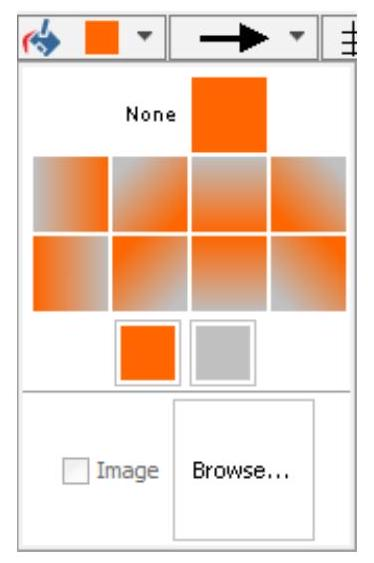
\includegraphics[max width=\textwidth]{2022_12_20_3e2ffe6ad124ec91ee5cg-33}
\end{center}

\begin{enumerate}
  \setcounter{enumi}{3}
  \item To change the line color, select a color from the $\square$ menu.
\end{enumerate}

\begin{center}
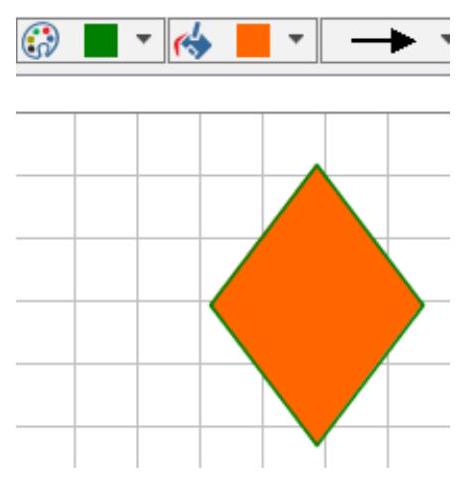
\includegraphics[max width=\textwidth]{2022_12_20_3e2ffe6ad124ec91ee5cg-33(1)}
\end{center}

\section{Filling an Object with a Gradient Color}
\section{To fill an object with a gradient color:}
\begin{enumerate}
  \item Select the object in the canvas.

  \item From the $\quad \nabla$ menu, select one of the gradient fill styles, the square icons.

  \item From the same menu, click the left and right color bars at the bottom to select a color from the color palette for each part of the gradient.

\end{enumerate}

\begin{center}
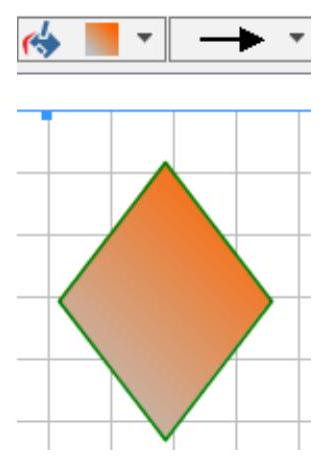
\includegraphics[max width=\textwidth]{2022_12_20_3e2ffe6ad124ec91ee5cg-34}
\end{center}

See below for instructions on filling an object with an image.

\subsection{Creating Hyperlinks}
You can add a hyperlink to a worksheet that links to another Maple Flow worksheet, a webpage, and more.

To insert a hyperlink:

\begin{enumerate}
  \item In a text container, select Insert>Hyperlink. The Hyperlink Properties dialog opens.

  \item For the Link Text field, enter the text to be shown.

  \item Select the link type.

  \item For the Target field, enter the destination. Note that you have to save your document if you want to use a relative path.

  \item Optionally, you can add a hyperlink tooltip.

\end{enumerate}

You can also create a hyperlink by selecting some text and using the Format $>$ Convert $>$ Hyperlink menu item.

To edit the hyperlink properties, right-click the hyperlink and select Hyperlink Properties from the context menu.

You can create a hyperlink to a Maple Flow help page. For example, setting Type to Help Topic and Target to solve creates a link to the solve help page.

\begin{center}
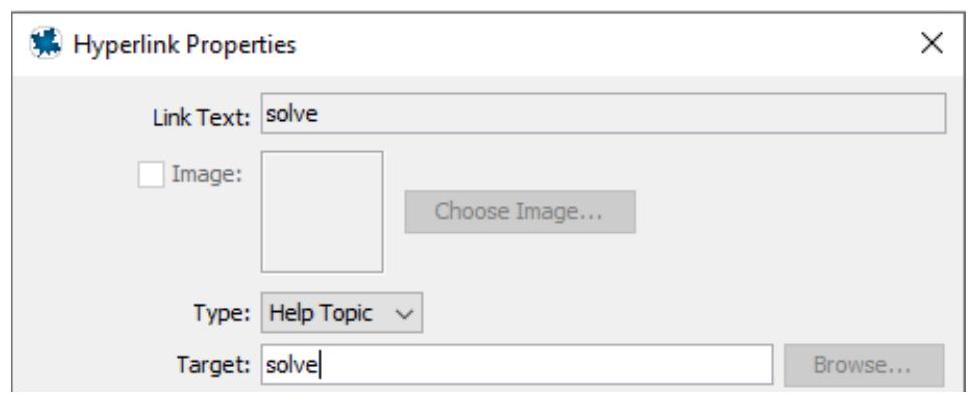
\includegraphics[max width=\textwidth]{2022_12_20_3e2ffe6ad124ec91ee5cg-34(1)}
\end{center}

Figure 4.10: Help Topic Hyperlink

In addition to hyperlinks, your worksheet can contain shortcut components, which are clickable image links. The default look of a shortcut is shown in Figure 4.11, but you can change the image used. The Application Gallery in Maple Flow uses shortcuts.

\begin{center}

\includegraphics[max width=\textwidth]{2022_12_20_3e2ffe6ad124ec91ee5cg-35}
\end{center}

Shortcut

Figure 4.11: Shortcut

To insert a shortcut:

\begin{enumerate}
  \item Click on the canvas.

  \item Select Insert $>$ Shortcut. A shortcut component is inserted at the cursor.

  \item To edit the shortcut properties, select the shortcut component, and in the Context Panel the shortcut properties are available.

\end{enumerate}

\begin{center}
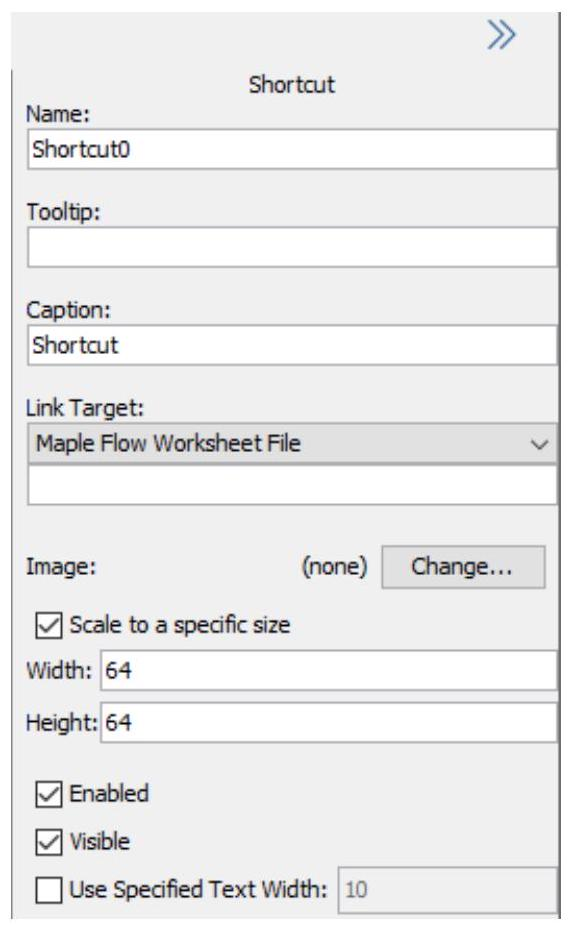
\includegraphics[max width=\textwidth]{2022_12_20_3e2ffe6ad124ec91ee5cg-35(1)}
\end{center}

Figure 4.12: Shortcut Properties

\begin{enumerate}
  \setcounter{enumi}{3}
  \item Specify a caption, which appears below the image. Optionally, add a tooltip. Note: The Name field is used by Maple Flow to identify the component. The caption is what is visible.

  \item Specify a link target. You can link to a Maple Flow worksheet or URL. You can also use the Shortcut to open a blank Maple Flow worksheet,

  \item If desired, change the image.

\end{enumerate}

\section{Further Tools: Mathematical Functions, Programming, and Plots}
\subsection{Mathematical Functions}
\section{Maple Functions}
Maple Flow is built on top of the Maple programming language. You can use most Maple functions in Maple Flow.

Maple package functions are used in the long form. For example, SignalProcessing:-FFT(). Note: Use of the with() command to load packages is not supported.

The Maple programming language is described in the Maple online help: \href{http://www.maplesoft.com/support/help}{http://www.maplesoft.com/support/help}.

\section{Unsupported Maple Keywords, Commands, and Packages}
As noted above, the with 0 command is not supported, and instead package commands should be called using the long form of their name. In addition, some Maple keywords, commands, and packages are not supported. The following are some examples, but not a complete list.

The assume command is not supported (use assuming instead). Some keywords, such as read and save, are not supported.

These Maple packages are not supported:

\begin{itemize}
  \item Physics

  \item Tolerances

  \item DocumentTools

  \item Typesetting

\end{itemize}

Procedures can only be defined in the Code Editor. See Code Editor (page 31).

\subsection{Plots}
You can create a plot with the Maple language plot command. A simple example is given in Figure 5.1.

\begin{center}
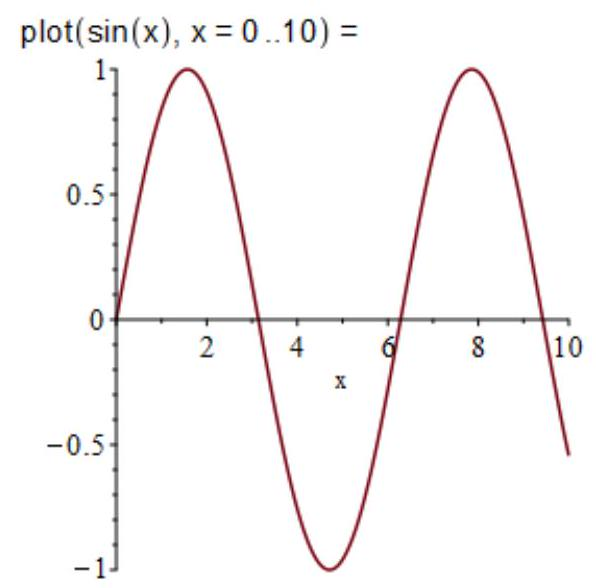
\includegraphics[max width=\textwidth]{2022_12_20_3e2ffe6ad124ec91ee5cg-36}
\end{center}

Figure 5.1: A simple plot using a Maple plot command

Plots can be rotated in the same way that drawings are rotated. To rotate the plot:

\begin{enumerate}
  \item Select the plot container with the selection tool. The vertices of the plot container are designated by grab boxes.

  \item Place the cursor at one of the vertices.

  \item Press Ctrl. The rotate icon is displayed.

  \item While pressing Ctrl, click the mouse and drag. The plot container rotates. Release the mouse once the object is positioned as you want.

\end{enumerate}

\subsection{Command Completion}
Maple Flow offers a dialog for command completion. Maple Flow suggests commands and parameters that complete what you have already entered.

The command completion dialog is initiated by pressing Esc or Ctrl + Space.

fs

fscanf

fscr $\quad f$

fsolve $\quad$ fsolve

fsolve $\quad$ fsolve(eqn)

fsolve (equation set) $\quad$ fsolve( ( eqn 1, eqn $2, \ldots\})$

fsolve (equation set, complex solutions) fsolve( (eann 1, eqn $2, \ldots\}$, complex')

Figure 5.2: Command completion window

\subsection{Code Editor}
The Code Editor lets you write Maple procedures to use in a Maple Flow canvas. To learn how to write a Maple procedure, read the online Maple Programming Guide:

\href{https://www.maplesoft.com/support/help/Maple/view.aspx?path=ProgrammingGuide/Contents}{https://www.maplesoft.com/support/help/Maple/view.aspx?path=ProgrammingGuide/Contents}

To view the code editor, click the Code Editor button on the main toolbar, as illustrated in Figure 5.3. Alternatively, from the Edit menu, select Code.

\begin{center}

\includegraphics[max width=\textwidth]{2022_12_20_3e2ffe6ad124ec91ee5cg-37}
\end{center}

Figure 5.3: Code Editor button on main toolbar

Note: You can only enter proc definitions in the code editor. That is, your code should be in the form:

FirstProc: $=$ proc $(\ldots) \quad \ldots$ end proc;

NextProc:=proc (...) $\ldots$ end proc;

To define the procedure, enclose a sequence of statements between proc(...) and end proc statements, and specify the parameter name(s) in the parentheses after the proc statement. For example, a simple definition for a procedure that takes one parameter and returns the square of the parameter is:

MyProc: $=\operatorname{proc}(\mathrm{x}) \mathrm{x}^{\wedge} 2$; end proc;

\section{Printing and Exporting to PDF}
\subsection{Print Extents}
Selecting View $>$ Print Extents displays dashed horizontal and vertical lines. These indicate the extents of a printable page, taking into account the chosen page size, margins and headers/footers. Pages are printing column-by-column.

\begin{center}
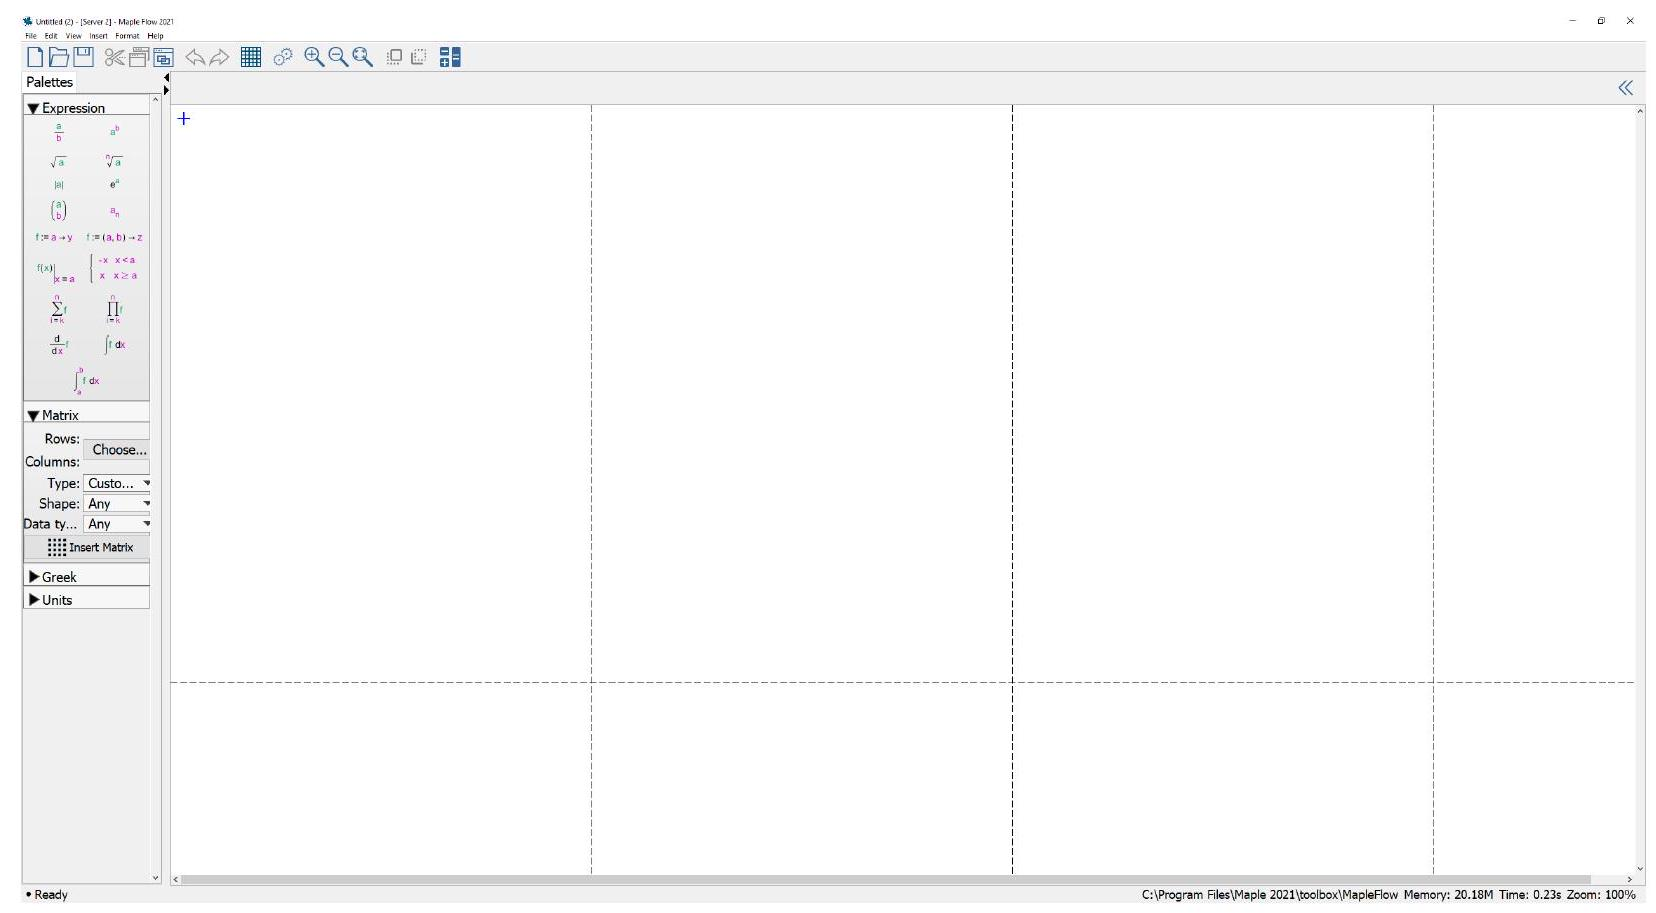
\includegraphics[max width=\textwidth]{2022_12_20_3e2ffe6ad124ec91ee5cg-38}
\end{center}

Figure 6.1: Print extents

The on-screen positioning and size of math, text, plots and images will be reflected in the printed page or exported PDF.

\subsection{Headers/Footers}
The Insert $>$ Header Footer menu lets you specify a header and/or footer. This will be seen in the printed page or exported PDF, but not in the working environment.

\begin{center}
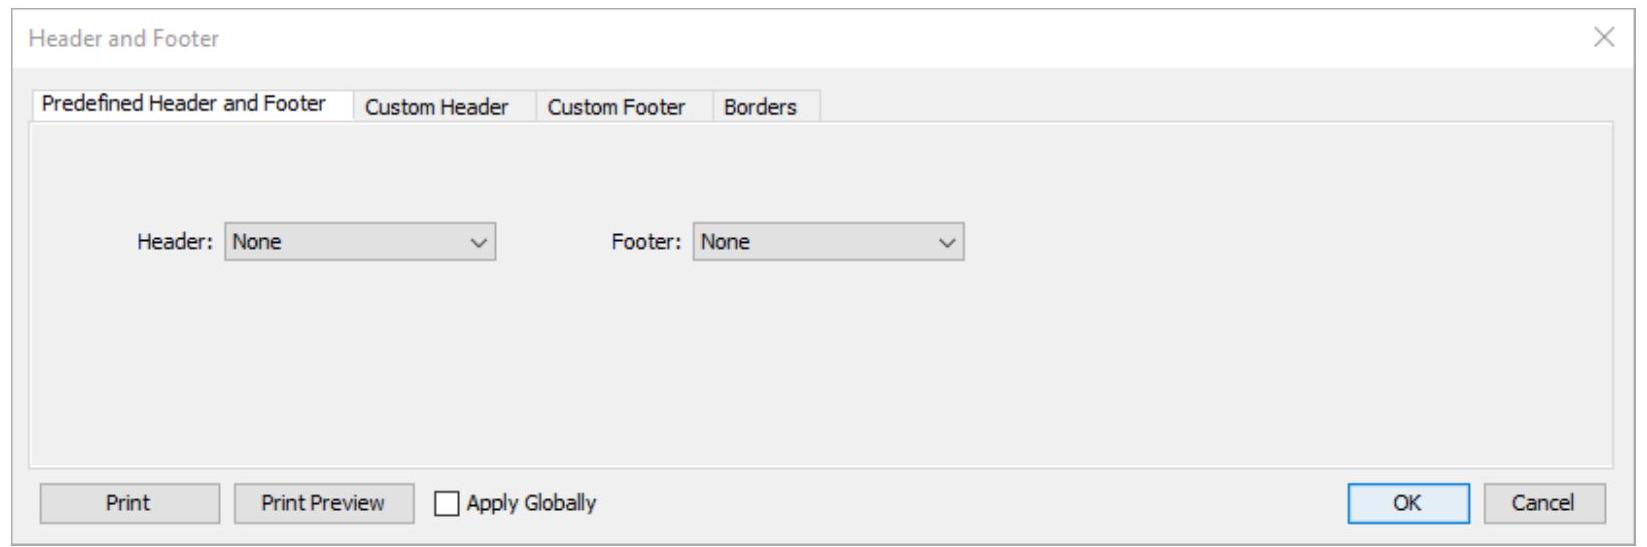
\includegraphics[max width=\textwidth]{2022_12_20_3e2ffe6ad124ec91ee5cg-38(1)}
\end{center}

Figure 6.2: Inserting Headers and Footers

\subsection{Page Setup and Print Preview}
The File $>$ Page Setup menu lets you change the page size, orientation, and margins, for printing.

\begin{center}
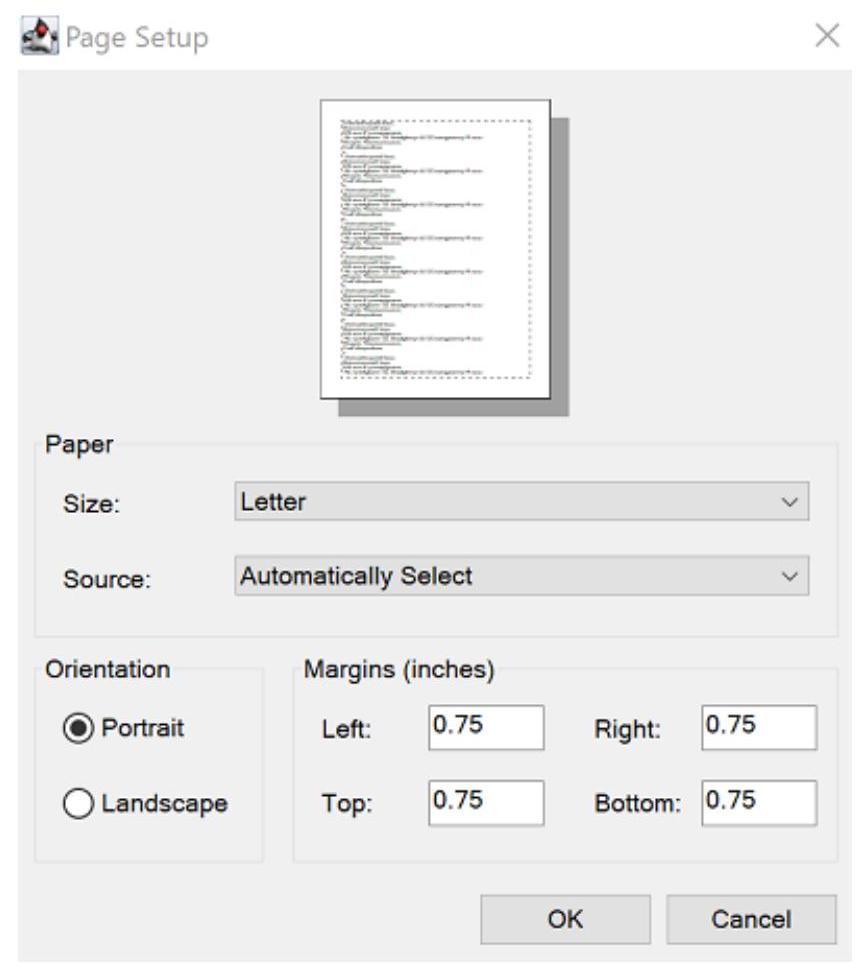
\includegraphics[max width=\textwidth]{2022_12_20_3e2ffe6ad124ec91ee5cg-39}
\end{center}

Figure 6.3: Page Setup

The File $>$ Print Preview menu lets you preview the printed page or exported PDF.

\subsection{Export to PDF}
To export the canvas to a PDF, click Print $>$ Export.

\subsection{Printing a Worksheet with Sections}
Whether printing or exporting to PDF, if your Maple Flow worksheet has sections, you can select how it is printed.

When you select Print or Print Preview, the Section Options for Print and PDF dialog opens. Select one of the following:

\begin{itemize}
  \item Print/export document with all sections expanded.

  \item Print/export document keeping sections exactly as shown on-screen.

\end{itemize}

If you selected the first option, in addition, specify whether to print the section boundary markers.

For more information on controlling the display of sections, see Controlling the Display of Sections (page 19).

\section{Keyboard Shortcuts}
Table 7.1: Keyboard shortcuts

\begin{center}
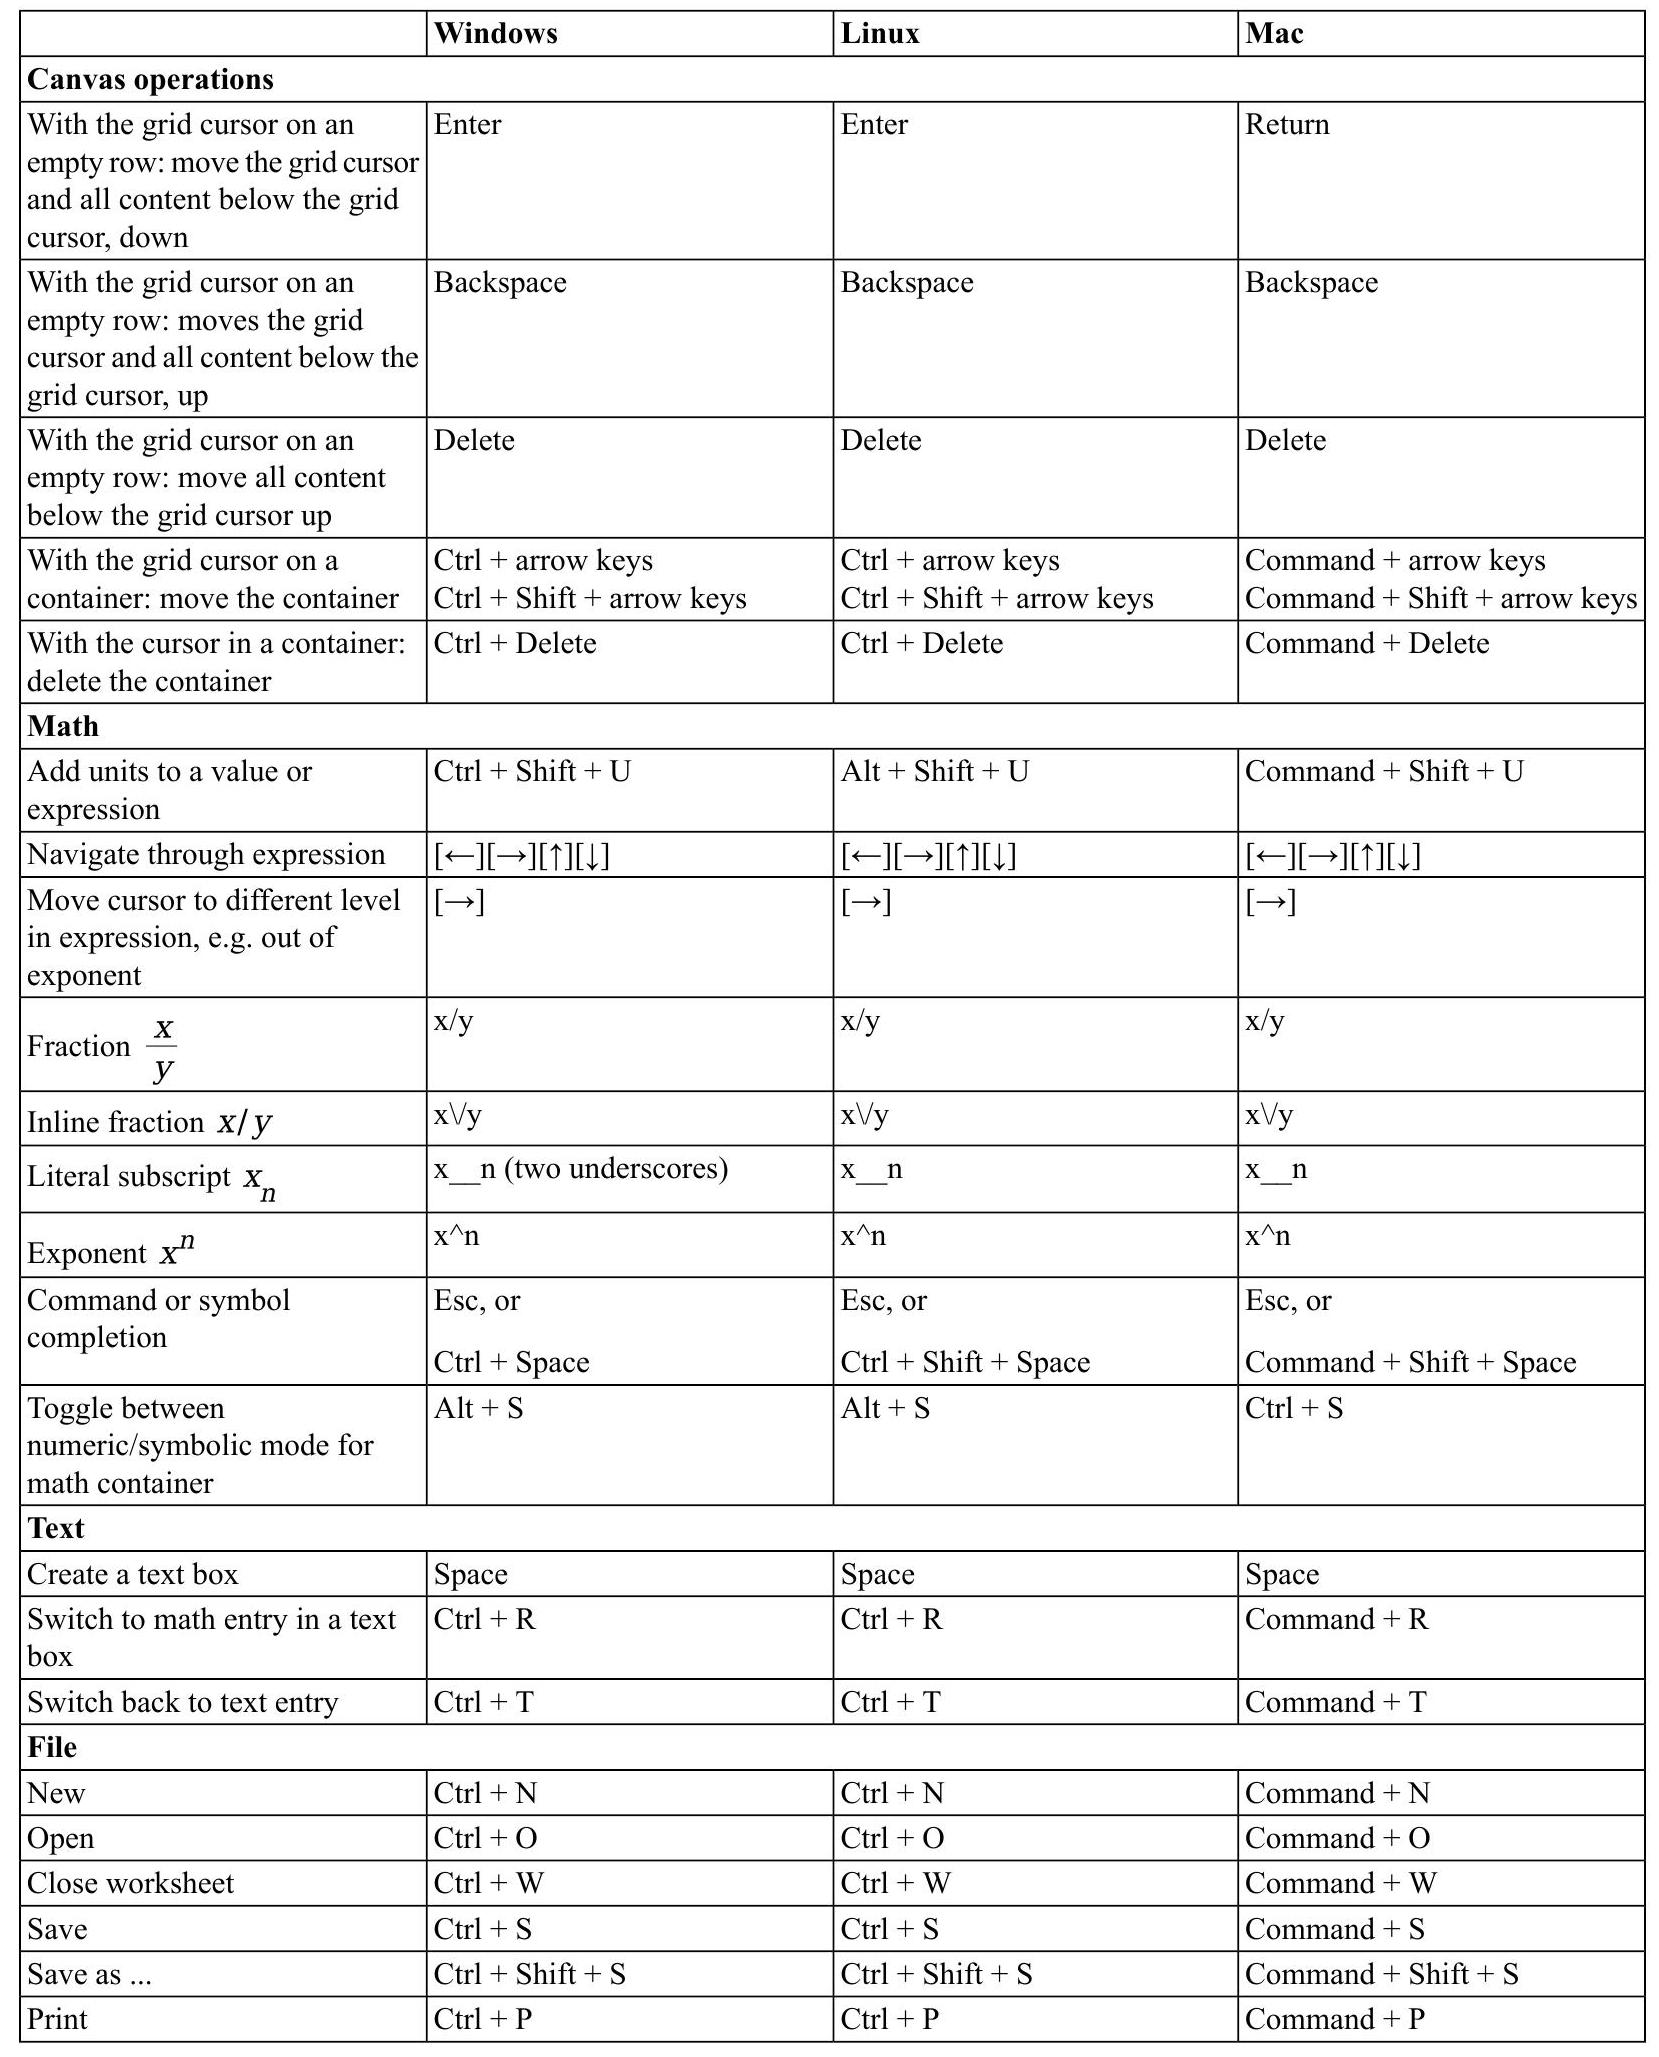
\includegraphics[max width=\textwidth]{2022_12_20_3e2ffe6ad124ec91ee5cg-40}
\end{center}

\begin{center}
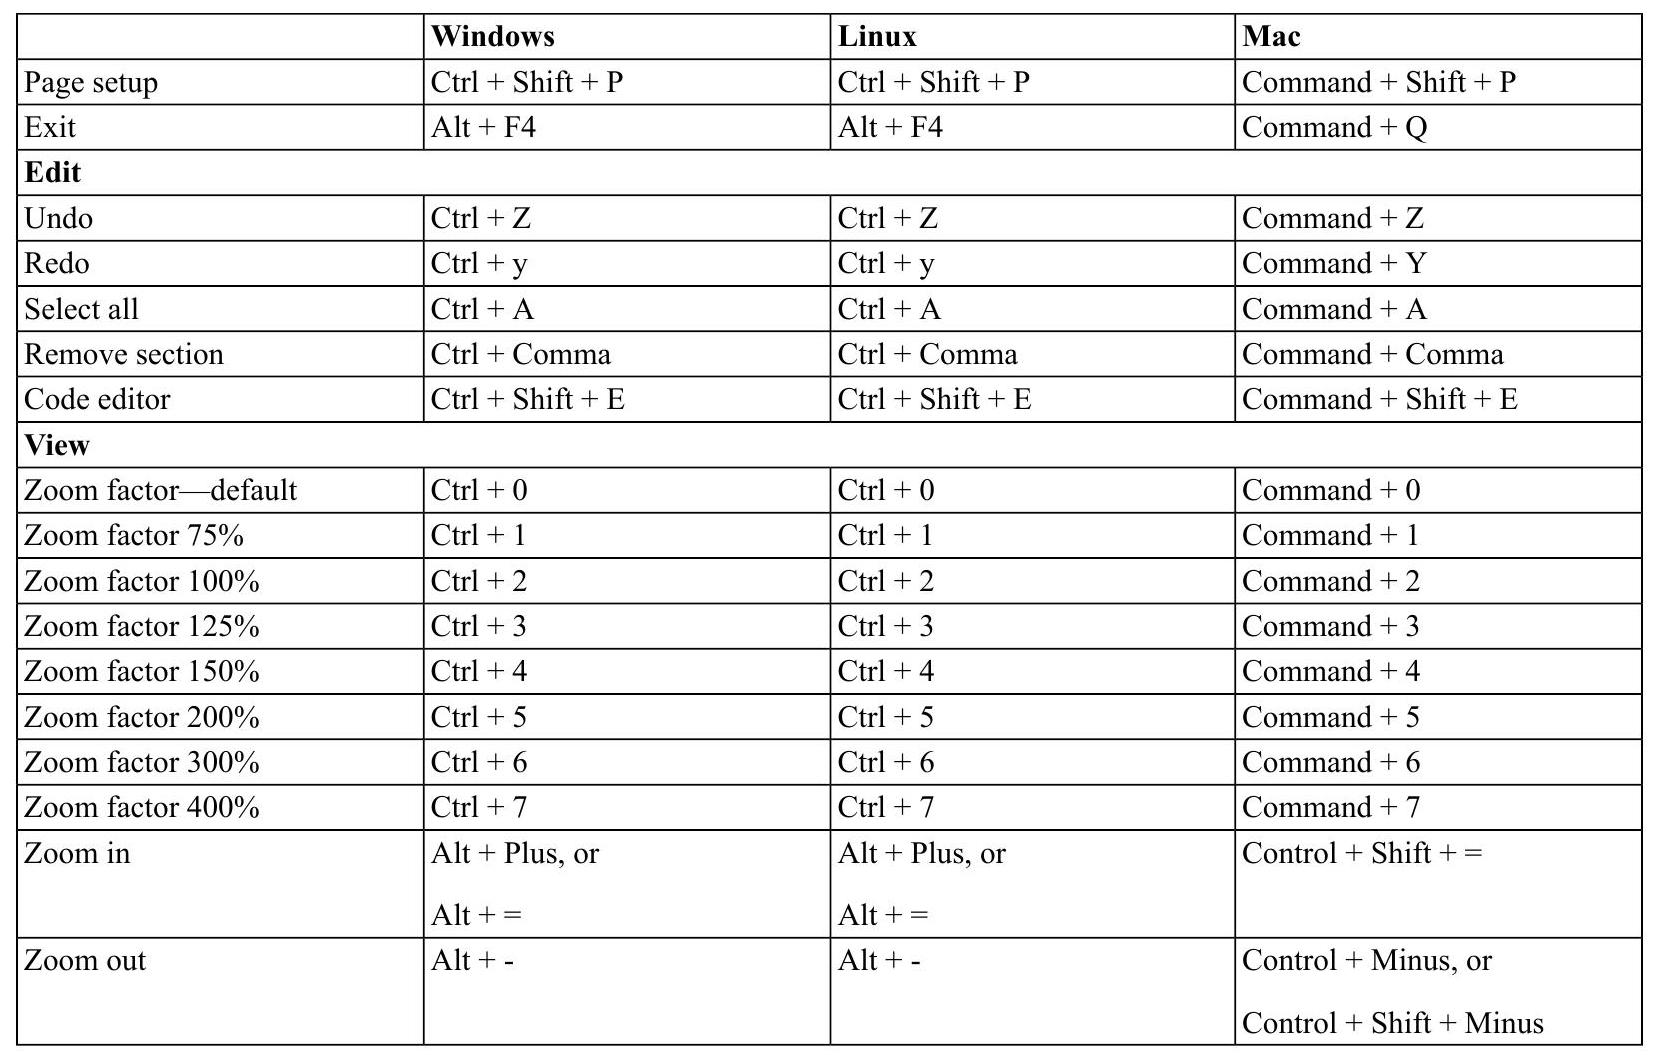
\includegraphics[max width=\textwidth]{2022_12_20_3e2ffe6ad124ec91ee5cg-41}
\end{center}

\section{Index}
\section{Symbols}
$:=, 11$

$=, 9$

